\section{Etherless-smart}

\subsection{Overview}
	Etherless-smart is the module which handles transactions on the Ethereum blockchain. It consists of a set of Ethereum smart contracts that handle the communication between Etherless-cli and Etherless-server as well as the payment of this work using ETH currency.

\subsection{Architecture} % Descrizione dell'architettura utilizzata, compresi i design pattern
		Our goals when developing Etherless-smart were upgradeability and extensibility. For these reasons said module consists of three separate smart contracts:
		\begin{itemize}
			\item \textbf{EtherlessSmart:} is the main contract which serves as the middleman between Etherless-cli and Etherless-server. Each one of its methods is either invoked by Etherless-cli to send the requests or by Etherless-server to transmit the responses. In order to complete its own function executions this contract contains an instance of the other two contracts and communicates with them via function calls;
			\item \textbf{EtherlessStorage:} is the storage contract. It stores all relevant information regarding the Javascript functions which can be called when using \textit{Etherless}. Moreover, it contains some utility methods to perform useful operations on this data;
			\item \textbf{EtherlessEscrow:} is the contract which manages everything in regards to monetary transactions. It contains details about every pending transaction and its methods have been implemented to manage an escrow payment.
		\end{itemize}

%Descrizione accurata dei metodi presenti nel modulo
\subsubsection{EtherlessSmart}
	\begin{figure}[H]
		\centering
		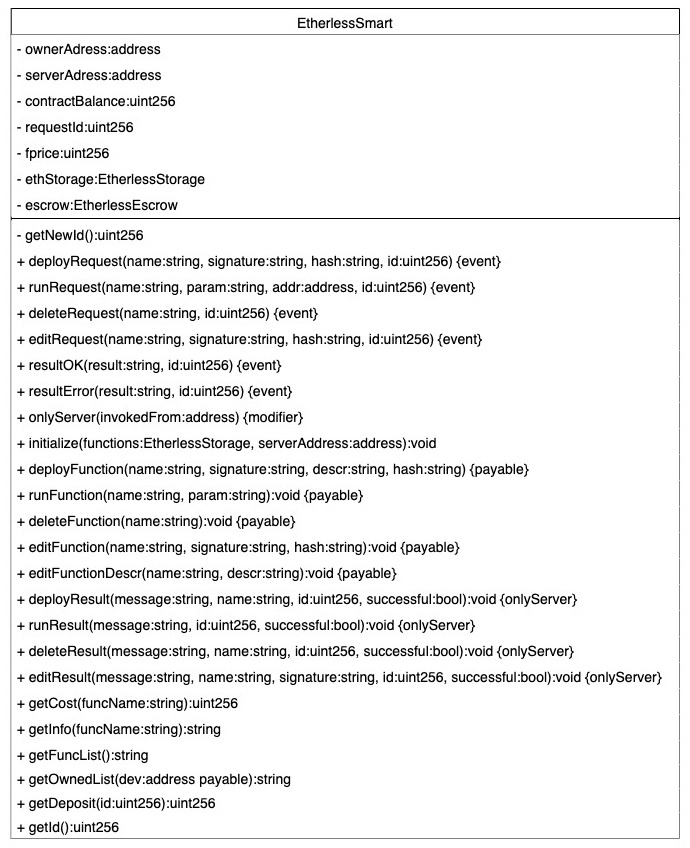
\includegraphics[width=0.6\linewidth]{diagrammi/etherless-smart/EtherlessSmart.jpg}
		\caption{Class diagram of EtherlessSmart}
	\end{figure}

\subsubsubsection*{Attributes}
	\begin{itemize}
		\item \textbf{ownerAddress:} address of the EtherlessSmart contract;
		\item \textbf{serverAddress:} server address;
		\item \textbf{contractBalance:} amount of ETH stored in the smart contract;
		\item \textbf{requestId:} unique identifier used to mark each request that needs payment;
		\item \textbf{ethStorage:} instance of EtherlessStorage contract;
		\item \textbf{escrow:} instance of EtherlessEscrow contract;
	\end{itemize}
\subsubsubsection*{Modifiers}
	\begin{itemize}
		\item \textbf{onlyServer:} restricts the access only to the server address.
	\end{itemize}
\subsubsubsection*{Events}
	\begin{itemize}
		\item \textbf{runRequest:} event emitted when a request of a function execution is received;
		\item \textbf{deployRequest:} event emitted when a request of a function deployment is received;
		\item \textbf{editRequest:} event emitted when a request of a function modification is received;
		\item \textbf{deleteRequest:} event emitted when a request of a function deletion is received;
		\item \textbf{resultOK:} event emitted when the result of a certain execution has to be communicated;
		\item \textbf{resultError:} event emitted when the failure of a certain execution has to be communicated;
	\end{itemize}
\subsubsubsection*{Methods}
	\begin{itemize}
		\item \textbf{deployFunction:} requests the deployment of a certain function;
		\item \textbf{runFunction:} requests the execution of a certain function;
		\item \textbf{editFunction:} requests the modification of a certain function;
		\item \textbf{deleteFunction:} requests the deletion of a certain function; can only be invoked by the developer of said function;
		\item \textbf{deployResult:} communicates the result of a function deployment; can only be invoked by the server address;
		\item \textbf{runResult:} communicates the result of a function execution; can only be invoked by the server address;
		\item \textbf{editResult:} communicates the result of a function modification; can only be invoked by the server address;
		\item \textbf{deleteResult:} communicates the result of a function deletion; can only be invoked by the server address;
		\item \textbf{getCost:} returns the cost of execution of a function;
		\item \textbf{getInfo:} returns all the information regarding a certain function;
		\item \textbf{getFuncList:} returns the names of all functions that have been deployed;
		\item \textbf{getOwnedList:} returns the names of all functions that have been deployed by a certain developer;
		\item \textbf{getNewId:} returns \texttt{requestId} incremented by one;
		\item \textbf{getId:} returns \texttt{requestId}.
	\end{itemize}

\subsubsection{EtherlessStorage}
	\begin{figure}[H]
		\centering
		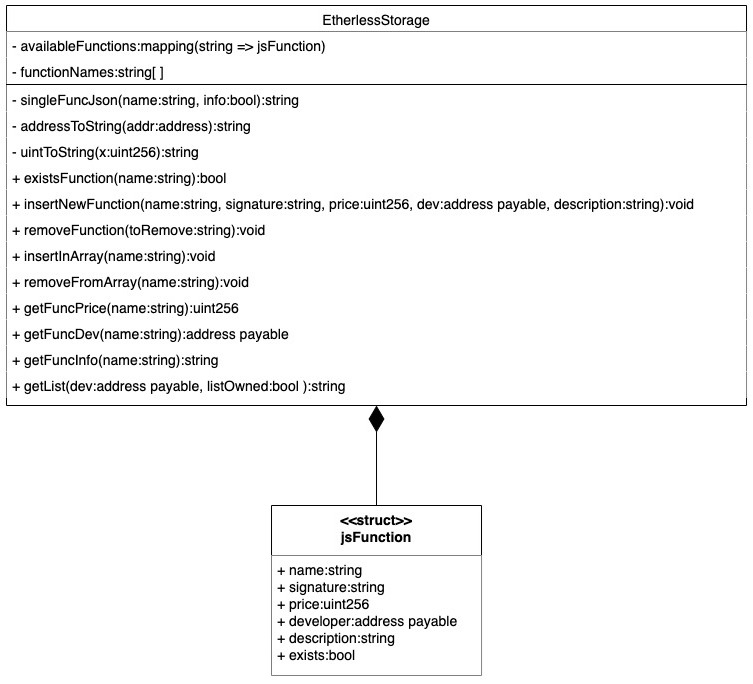
\includegraphics[width=0.6\linewidth]{diagrammi/etherless-smart/EtherlessStorage.jpg}
		\caption{Class diagram of EtherlessStorage}
	\end{figure}

\subsubsubsection*{Attributes}
	\begin{itemize}
		\item \textbf{availableFunctions:} mapping that stores details regarding all functions that have been deployed. Each entry is a key-value pair where the key is the name of the function and the value is a \texttt{jsFunction} struct;
		\item \textbf{functionNames:} array containing the names of all functions that have been deployed. The existence of this array is required since the key value of the \texttt{availableFunctions} mapping cannot be used to perform logical operations.
	\end{itemize}
\subsubsubsection*{Methods}
	\begin{itemize}
		\item \textbf{singleFuncJson:} converts the content of a \texttt{jsFunction} struct into a string written in JSON format;
		\item \textbf{addressToString:} converts an address into a string;
		\item \textbf{uintToString:} converts an unsigned integer into a string;
		\item \textbf{existsFunction:} checks if a function is in \texttt{availableFunctions};
		\item \textbf{insertNewFunction:} adds a function to the \texttt{availableFunctions} mapping;
		\item \textbf{removeFunction:} removes a function from the \texttt{availableFunctions} mapping;
		\item \textbf{insertInArray:} adds a function to the \texttt{functionNames} array;
		\item \textbf{removeFromArray:} removes a function from the \texttt{functionNames} array;
		\item \textbf{getFuncPrice:} returns the price of execution of a certain function;
		\item \textbf{getFuncDev:} returns the developer address of a certain function;
		\item \textbf{getList:} returns the name of all functions a user can execute when using \textit{Etherless};
		\item \textbf{getFuncInfo:} returns all information regarding a function;
		\item \textbf{compareString:} compares two strings using a reasonable gas amount.
	\end{itemize}

\subsubsection{EtherlessEscrow}
	\begin{figure}[H]
		\centering
		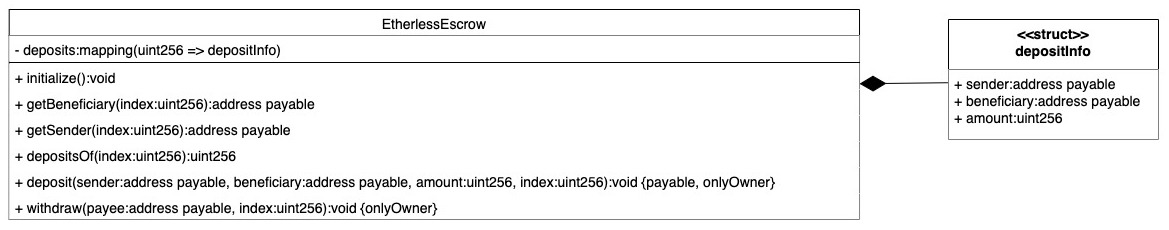
\includegraphics[width=1\linewidth]{diagrammi/etherless-smart/EtherlessEscrow.jpg}
		\caption{Class diagram of EtherlessEscrow}
	\end{figure}

\subsubsubsection*{Attributes}
	\begin{itemize}
		\item \textbf{deposits:} mapping that stores details regarding all pending transaction. Each entry is a key-value pair where the key is a unique identifier and the value is a \texttt{depositInfo} struct.	
		\end{itemize}
\subsubsubsection*{Methods}
	\begin{itemize}
		\item \textbf{getBeneficiary:} returns the beneficiary of the transaction from the \texttt{deposits} mapping having the key \texttt{index};
		\item \textbf{getSender:} returns the sender of the transaction from the \texttt{deposits} mapping having the key \texttt{index};
		\item \textbf{depositsOf:} returns the amount deposited in \texttt{deposits} identified by the key \texttt{index};
		\item \textbf{deposit:} stores the amount sent during a transaction, its sender and its beneficiary in \texttt{deposits} with the key value \texttt{index};
		\item \textbf{withdraw:} withdraws and sends the amount stored in the \texttt{deposits} mapping having the key \texttt{index} to the \texttt{payee} address.
	\end{itemize}

\newgeometry{a4paper,left=1in,right=1in,top=1in,bottom=1in,nohead}
	\begin{landscape}
	\subsection{UML}
		\begin{figure}[H]
			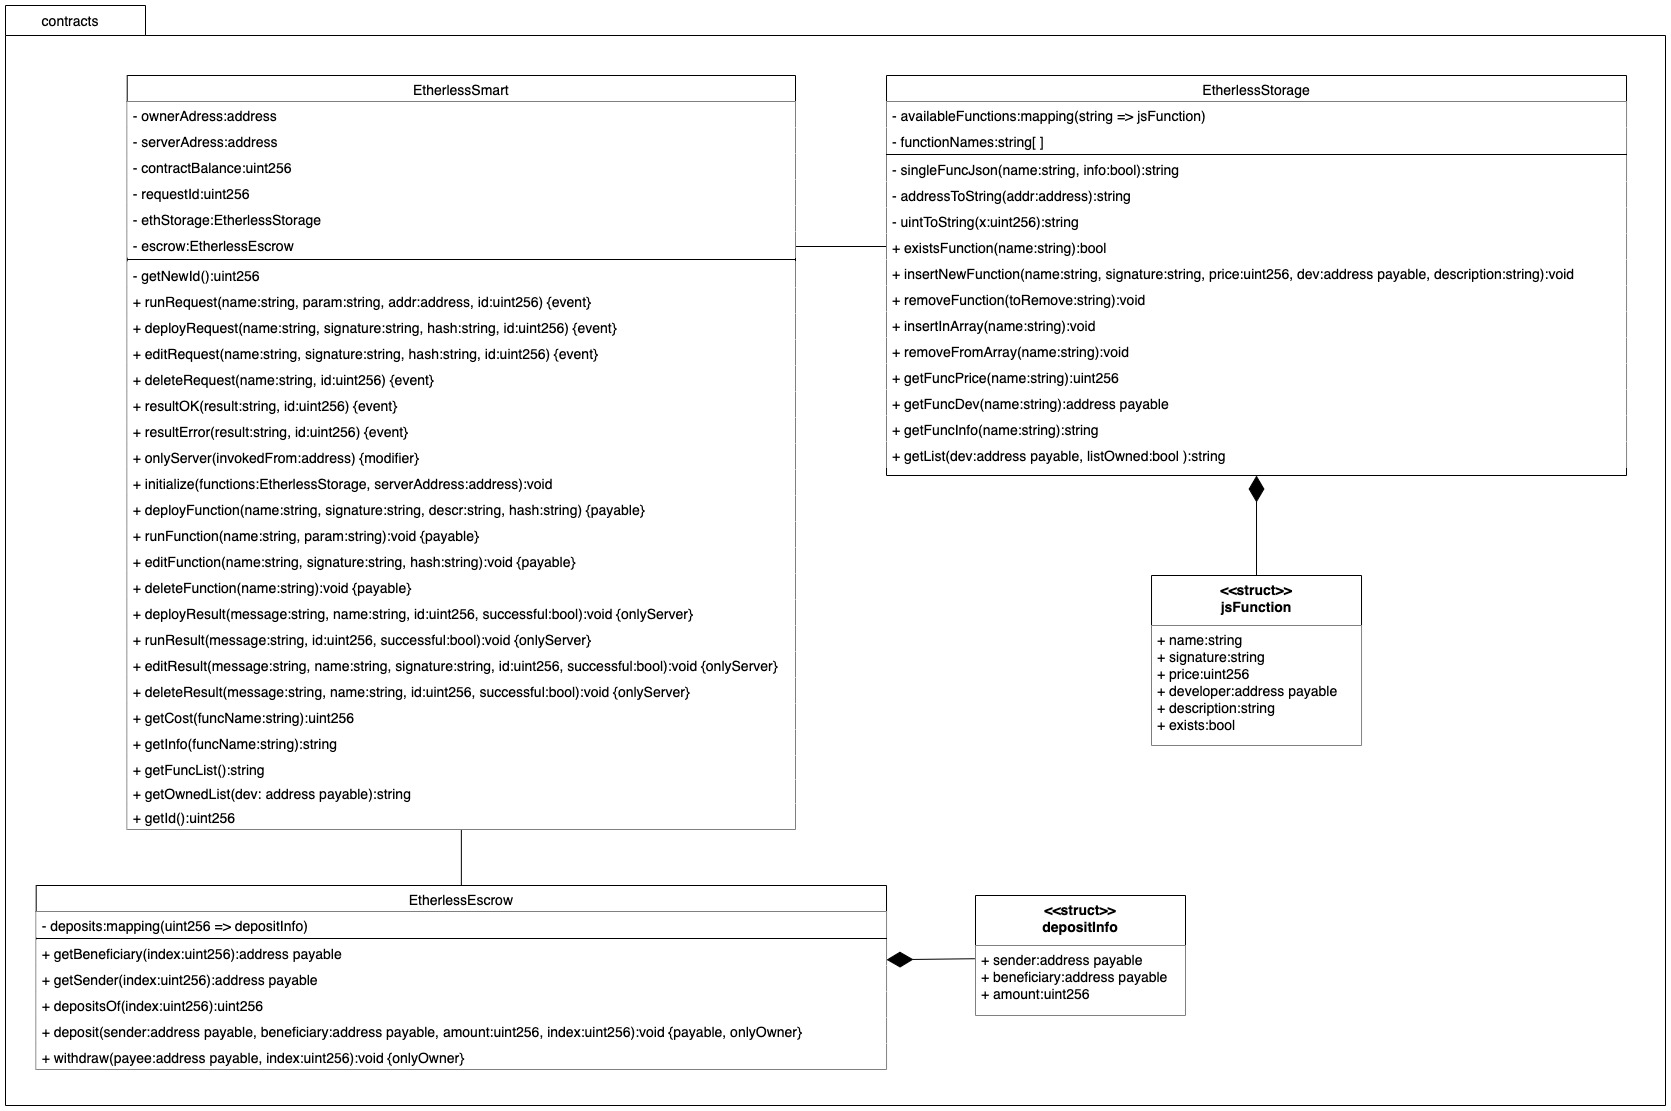
\includegraphics[width=21cm]{./diagrammi/etherless-smart/Etherless-smart.jpg}
			\caption{Etherless-smart module architecture.}
		\end{figure}
	\end{landscape}
	\restoregeometry

\subsection{Extensions}  %Possibili sviluppi futuri
As described above, smart contracts have been developed with the aim of being upgradable, meaning all the contracts can be updated without losing stored data. \\
To do this, we have decided to use the framework \textit{OpenZeppelin} because of its implementation under the hood of the proxy delegate pattern to upgrade smart contracts. \\
On the developer side, this makes the upgrade of a smart contract very simple. In order to upgrade a contract all the new features desired can be added without changing the order of the elements that are already there. Then, by typing \texttt{npx oz upgrade} in the terminal window, the smart contract will be upgraded. \\
For more information, the official documentation can be consulted here: \url{https://docs.openzeppelin.com/upgrades/2.6/}.
